\section{IR and Collinar Divergences}
Beyond the LO (Leading order) diagrams it happens singularities. To discuss about these consider first the process $ e^- e^+ \rightarrow q\bar{q}g $

\begin{figure}[ht!]
\centering
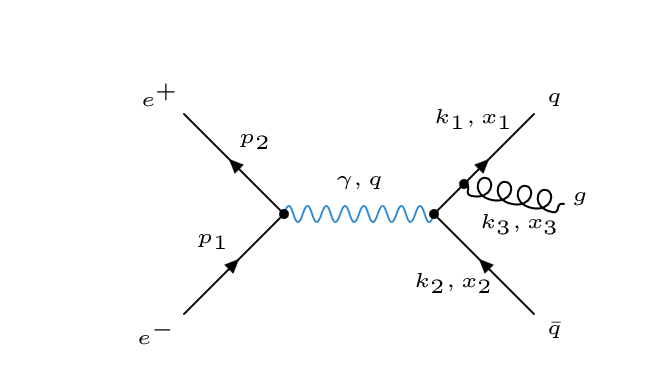
\includegraphics[width=0.85\textwidth]{images/Intro/IRCol.png}
\end{figure}
We define the energy fraction by:
\begin{equation}
x_i = \frac{2E_i}{\sqrt{s}}=\frac{2q\: \cdot\: k_i}{s}
\end{equation}
One can show that $ \sum x_i =2  $ and thus, that only two of the $ xi $ are independent.
In order to calculate the cross section of this diagram, we have to consider the gluon emission from the antiquark. Since the calculation is quite long, we concentrate on the final result, which can be found in almost every QCD lectures, e.g. H\&M Section 11.5.
\begin{figure}[ht!]
\centering
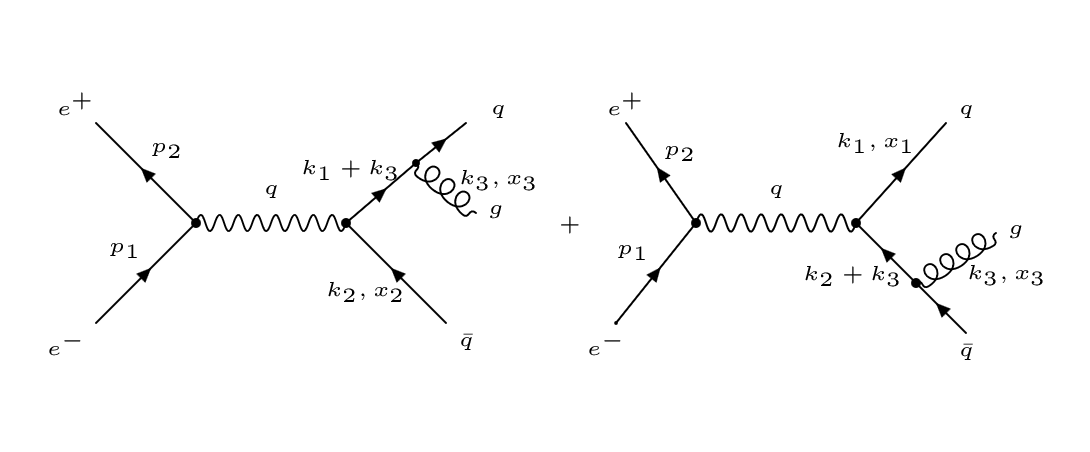
\includegraphics[width=0.85\textwidth]{images/Intro/IRColMatrix.png}
\caption{Left diagram $  e^- e^+ \rightarrow qg\bar{q} $ and right $ e^- e^+ \rightarrow q\bar{q}g $}
\end{figure}

The final result is:
\begin{equation}
\frac{d^2 \sigma}{dx_1 dx_2}= (\frac{4\pi \alpha}{s})\sum {e_i}^2 
\frac{2\alpha_s}{3\pi} \frac{{x_1}^2+{x_2}^2}{(1-x_1)(1-x_2)}
\end{equation}

There are three singularities in regard with the final result. 
If the emitted photon is collinear to the outgoing quark or anti-quark $ (x_1 \rightarrow 1 or x_2 \rightarrow 1) $ and When the emitted gluon is very soft $ (x_1 \rightarrow 1 and x_2 \rightarrow 1 )$.
The singularities come from the quark propagator in each diagram. The denominators contain according Feynmann rules terms with $\sim \frac{1}{(k_i + k_j)^2}  $. We can eliminate the quark mass under on-shell condition so that:
\begin{equation}
\frac{1}{(k_i + k_j)^2}=\frac{1}{2k_i \cdot k_j}=\frac{1}{2E_iE_j(1-cos\theta_{ij})}=\frac{1}{s(1- x_k)}
\end{equation} 
One can show all possibilities for three partons through a triangle:

\begin{figure}[ht!]
\centering
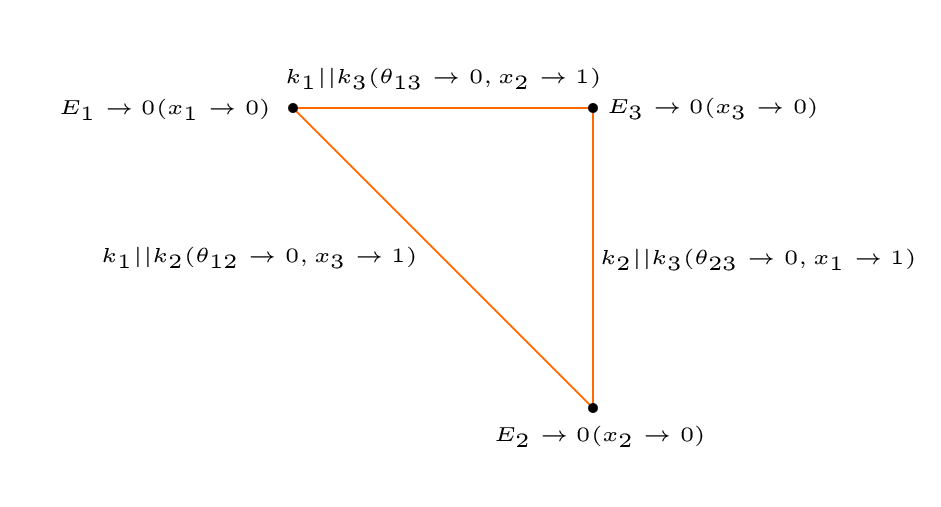
\includegraphics[width=0.85\textwidth]{images/Intro/triangle.png}
\end{figure}
We will use deep inelastic scattering (DIS) to show how the infrared singularities are absorbed in the parton distributions.
REAL and VIRT are separately divergent-could fix using splitting/subtraction method

\section{Factorisation}
The hadron hadron scattering can be written as:
\begin{equation}
\sigma = \sum_{ij} \int dx_1 dx_2 f_i(x_1, \mu^2)f_j(x_2, \mu^2) \sigma_{ij}(x_1, x_2, Q^2/\mu^2... )
\end{equation}
\begin{figure}[h!]
\centering
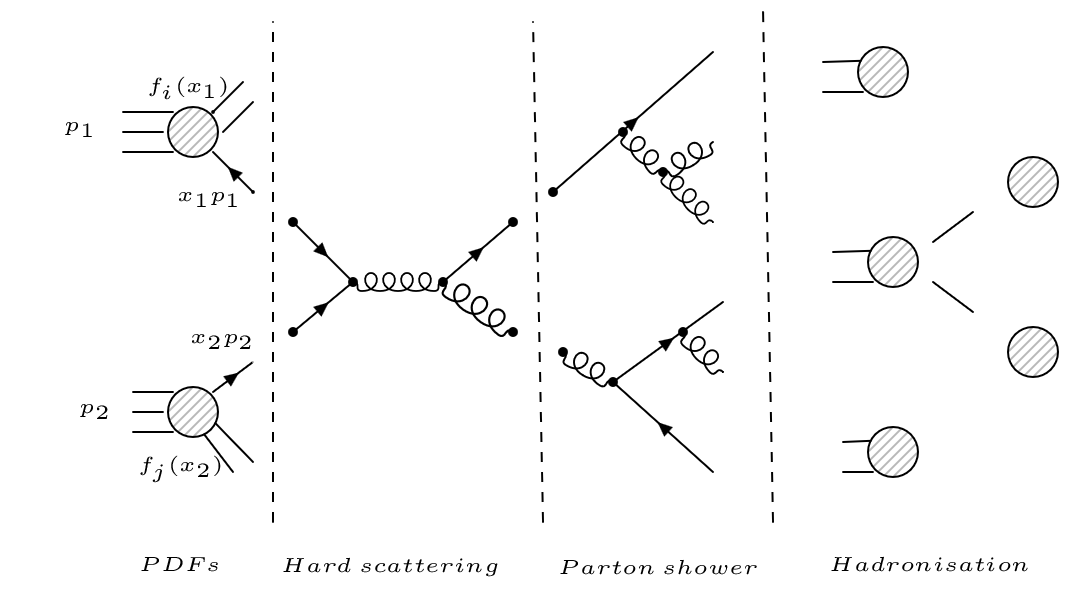
\includegraphics[width=0.85\textwidth]{images/Intro/Hard.png}
\end{figure}
Here the (arbitrary) factorisation scale $ \mu $ can be thought of
as the scale which separates the long and short-distance physics.
Roughly speaking, a parton with a transverse momentum less
than $ \mu $ is then considered to be part of the hadron structure and
is absorbed in the parton distribution. Partons with larger transverse
momenta participate in the hard scattering process with a
short-distance partonic cross-section.
The factorisation theorem also applies to deep inelastic scattering. The DIS cross section can be written as:
\begin{equation}
\frac{d^2 \sigma}{dx dQ^2}=\frac{4\pi \alpha^2}{x Q^4}[(1-y)F_2 (x, Q^2)+xy^2 F_1(x, Q^2)]
\end{equation}
In this case we need to introduce the structure function, is defined as the charge weighted sum of the parton momentum densities, the probability that the parton carries a momentum
fraction x. The index i denotes the quark. 
flavour.
\begin{equation}
{{F}_2}^{exp} (x)= \sum_i {e_i}^2 x f_i(x)
\end{equation}
The evolution of a quark
distribution due to gluon radiation and is called the DGLAP
evolution equation.
\begin{equation}
\frac{\partial f(x, \mu^2) }{\partial \: ln \:\mu^2}=
\frac{\alpha_s}{2\pi}\int_{x}^{1}\frac{dy}{y} f(y, \mu^2) P_{qq}(\frac{x}{y}+O({\alpha_s}^2)
\end{equation}
There three more spiriting possibilities according to below diagrams.

\begin{figure}[h!]
\centering
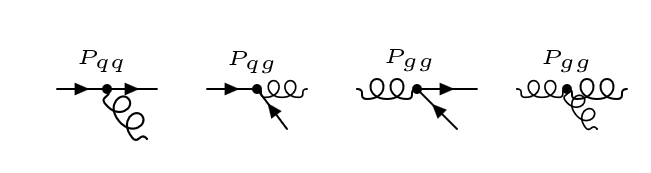
\includegraphics[width=0.85\textwidth]{images/Intro/spiliting.png}
\end{figure}

\begin{equation}
	\left.\begin{aligned}
\langle\:\hat{P_{qq}}\rangle &= C_F[\frac{1+z^2}{1-z}-\varepsilon(1-z)]\\
\langle\:\hat{P_{gq}}\rangle &= T_R[1-\frac{2z(1-z)}{1-\varepsilon}]\\
\langle\:\hat{P_{qg}}\rangle &= C_F[\frac{1+(1-z)^2}{z}-\varepsilon z]\\
\langle\:\hat{P_{gg}}\rangle &= 2C_A[\frac{z}{1-z}+\frac{1-z}{z}+z(1-z)]
\end{aligned}
	\right\}
	\quad \text{splitting functions}
\end{equation}

\section{splitting/subtraction method}

\section{Catani-Seymour Formalism}